\documentclass[xcolor=dvipsnames]{beamer}
\usecolortheme[named=PineGreen]{structure} 
\useoutertheme{infolines} 
\usetheme[height=7mm]{Rochester} 
\usefonttheme{structuresmallcapsserif}
\setbeamertemplate{items}[ball] 
\setbeamertemplate{blocks}[rounded][shadow=true] 
\setbeamertemplate{navigation symbols}{} 
\usepackage{tikz}

\newcommand{\authorquote}[2]{\begin{quote}``#2''\textnormal{~--~#1}\end{quote}}
\author{Wim Looman}
\title{Software Engineering}
\subtitle{In the Mariokart system}
\institute[UC]
{
  Department of Electrical Engineering\\
  University of Canterbury\\
  New Zealand
}
\date{26 September, 2011}

\begin{document}
  \begin{frame}[plain]
    \titlepage
  \end{frame}

  \begin{frame}{Outline}
    \begin{center}
      \begin{minipage}{0.5\linewidth}
        \tableofcontents
      \end{minipage}
    \end{center}
  \end{frame}

  \section{Continuous Integration}
    \subsection{What is it?}
      \begin{frame}{What is Continuous Integration?}
        \begin{definition}
          \authorquote{Martin Fowler\footnotemark}{%
            Continuous Integration is a software development practice where
            members of a team integrate their work frequently, usually each
            person integrates at least daily - leading to multiple integrations
            per day.  Each integration is verified by an automated build
            (including test) to detect integration errors as quickly as
            possible.%
          }
        \end{definition}
        \footnotetext{\url{http://martinfowler.com/articles/continuousIntegration.html}}
      \end{frame}

    \subsection{Why would you use it?}
      \begin{frame}{Why would you use Continuous Integration?}
      \end{frame}

    \subsection{CI Joe}
      \begin{frame}{CI Joe}
      \end{frame}

    \subsection{Did it help?}
      \begin{frame}{Did Continuous Integration help?}
      \end{frame}

    \subsection{Examples}
      \begin{frame}{Example 1}
        \only<1>{
          %
\includegraphics[width=0.45\linewidth]{images/green-dashboard}
          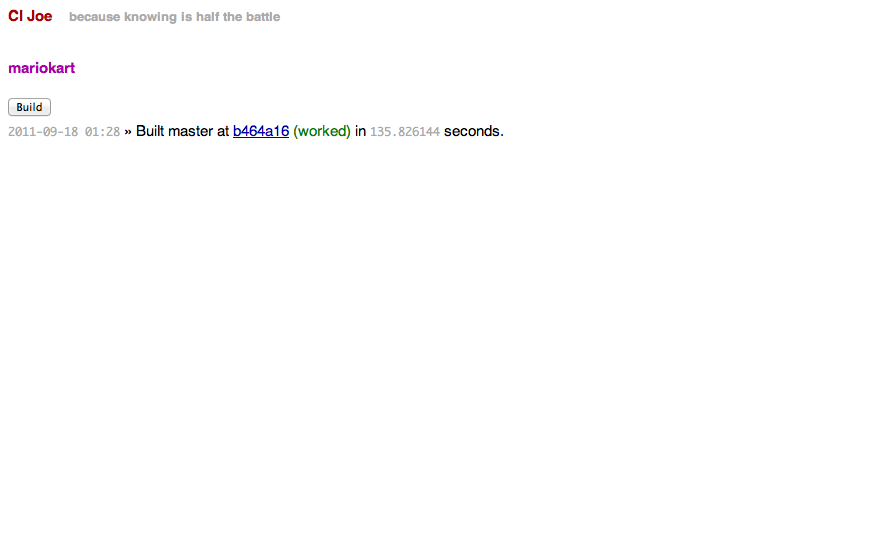
\includegraphics[width=\linewidth]{images/green-full}
        }
        \only<2>{
          %
\includegraphics[width=0.45\linewidth]{images/building-dashboard}
          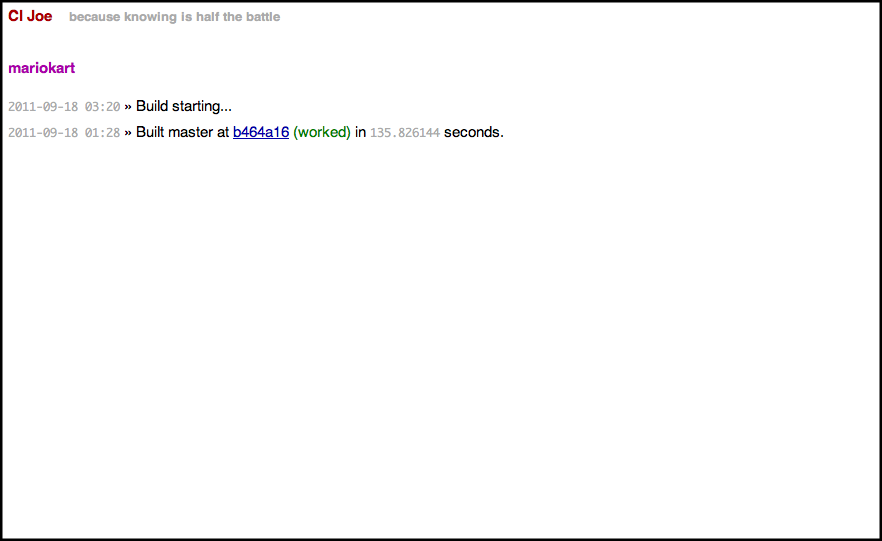
\includegraphics[width=\linewidth]{images/building-full}
        }
        \only<3>{
          %
\includegraphics[width=0.45\linewidth]{images/fail-dashboard}
          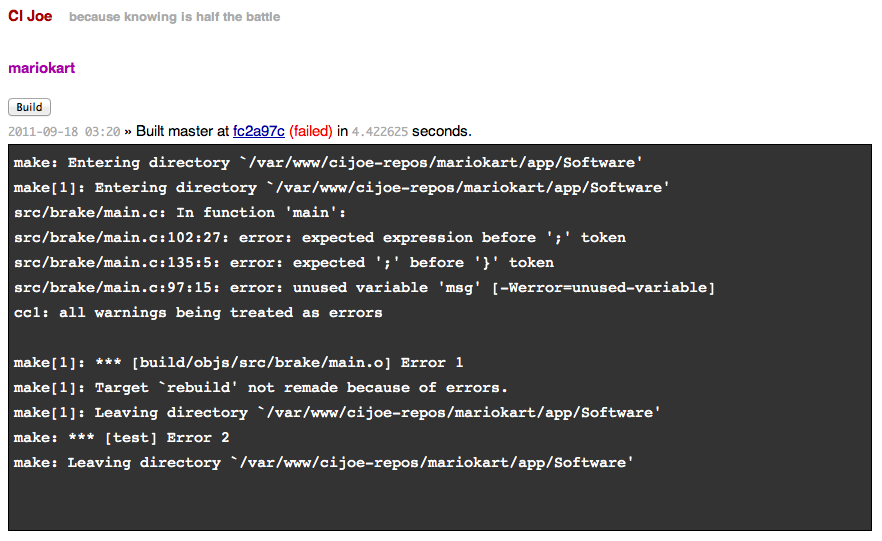
\includegraphics[width=\linewidth]{images/fail-full}
        }
      \end{frame}

      \begin{frame}{Example 2}
        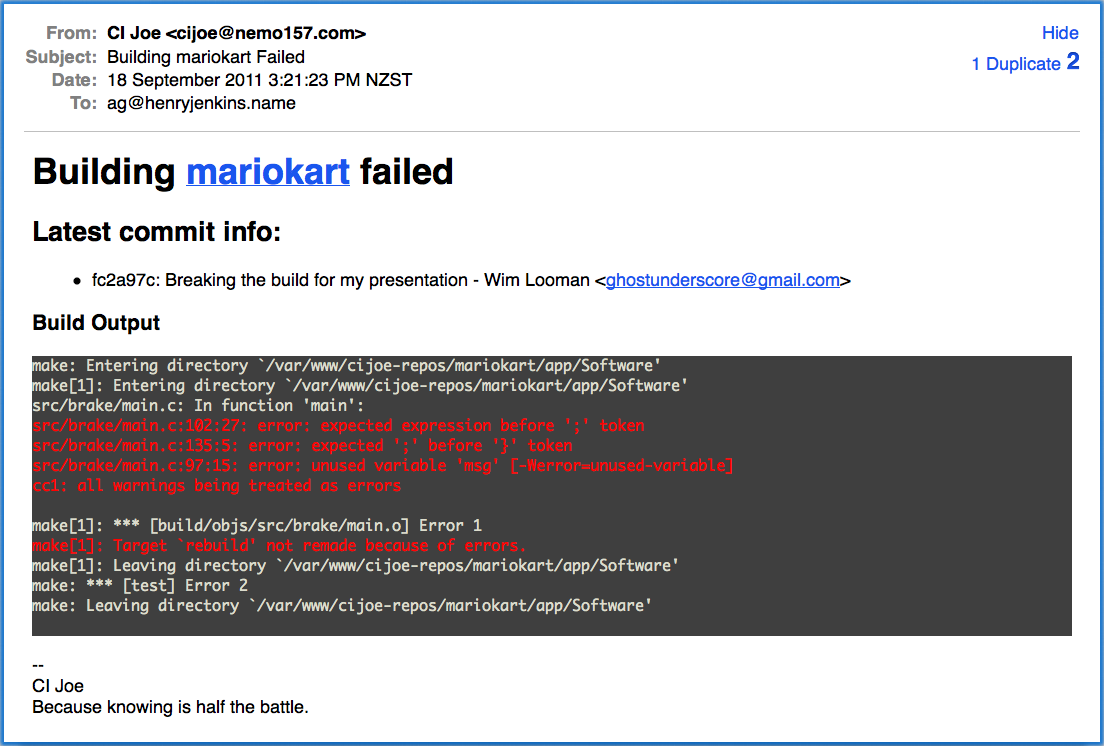
\includegraphics[width=\linewidth]{images/email}
      \end{frame}

    \section{Questions}
      \begin{frame}[plain]
        \begin{tikzpicture}[remember picture,overlay]
          \node[at=(current page.center)] {
            
\includegraphics[width=\paperwidth]{images/mario_kart_lego}
          };
        \end{tikzpicture}
      \end{frame}
\end{document}
